\section{Explainable models of agency}
This section deals with the application of XAI to Autonomous Agents (and Autonomous Planning).
\subsection{What is an agent?}
An agent is anything that can be viewed as perceiving its environment through sensors and
acting upon that environment through actuators. A human agent has eyes, ears, and other organs for sensors and hands, legs, vocal tract,
and so on for actuators. A robotic agent might have cameras and infrared range finders for
sensors and various motors for actuators.
We use the term percept to refer to the content an agent's sensors are perceiving. An
agent's percept sequence is the complete history of everything the agent has ever perceived.\\

We use the term percept to refer to the content an agent's sensors are perceiving. An
agent's percept sequence is the complete history of everything the agent has ever perceived.
Mathematically speaking, we say that an agent's behavior is described by the agent function that maps any given
percept sequence to an action.

\begin{center}
    \begin{minipage}[t]{0.3\textwidth}
        \begin{figure}[H]
            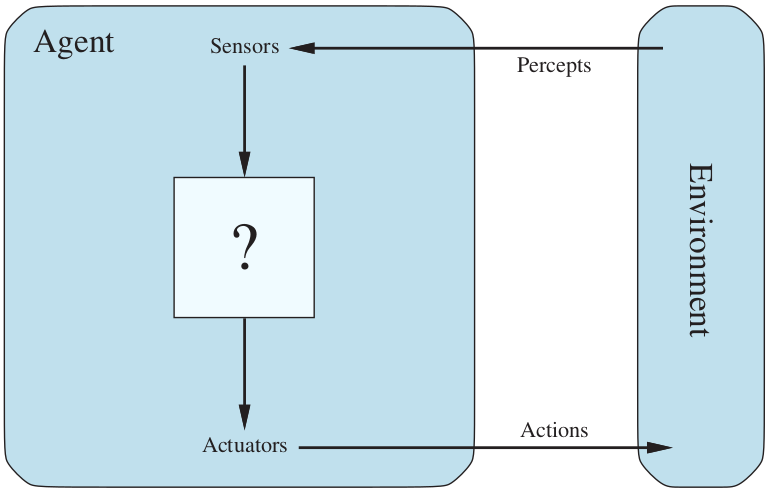
\includegraphics[width=\textwidth]{img/agent.png}
        \end{figure}
    \end{minipage}
    \hspace{2cm}
    \begin{minipage}[t]{0.4\textwidth}
        \begin{figure}[H]
            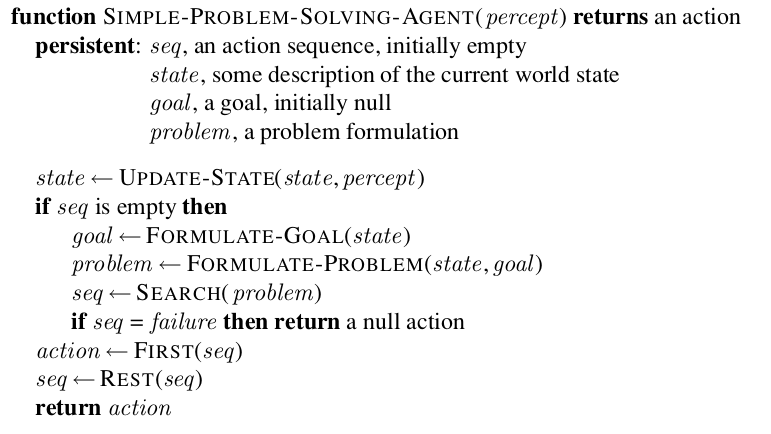
\includegraphics[width=\textwidth]{img/simpleprobsolving.png}
        \end{figure}
    \end{minipage}
\end{center}

A simple example of an autonomous agent and an environment is a robot playing chess.

How does humans play chess? 
\begin{itemize}
    \item We know the rules
    \item We observe the current state of the environment
    \item We \textbf{reason on the rules and the state}, and \textbf{infer} the next action (or even plan a short-term sequence)
\end{itemize}

This process of reason on the rules and the state is called Deductive Reasoning.
The definition of Deductive Reasoning is to infer facts from known other facts and rules.

\subsection{Logic}
A logic formalism is defined in terms of:
\begin{itemize}
    \item \textbf{Syntax}: symbols
    \item \textbf{Semantics}: the meaning of symbols
\end{itemize}
Formulas (or sentences) may be true or false depending on the value of variables
\begin{itemize}
    \item Sentence: $x+y=2$
    \item Model 1: $\{x=1,y=1\}\rightarrow$ sentence is true
    \item Model 2: $\{x=1,y=0\}\rightarrow$ sentence is false
\end{itemize}
A model $M$ is a possible assignment of all variables in a domain $D$.

The model of a formula $f$ in $D$, i.e., $M(f)$, is the set of assignments where $f$ holds.

\subsection{Propositional Logic}
\begin{figure}[H]
    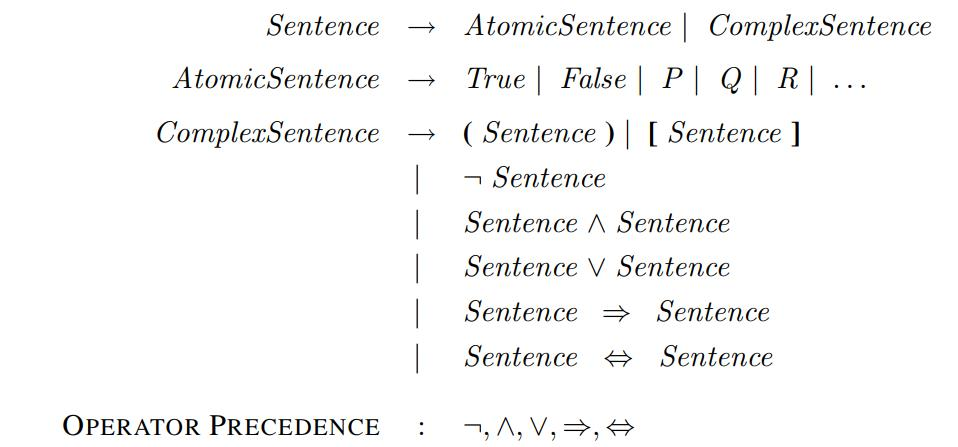
\includegraphics[width=0.7\textwidth]{img/proplogic.png}
    \centering
\end{figure}

\subsection{Logic Inference}

\begin{eqnarray*}
    \alpha \models \beta \text{ if and only if } M(\alpha)\subseteq M(\beta)\\
    \text{where } \alpha \text{ and } \beta \text{ are two formulas, } \\
    M(\alpha) \text{ and } M(\beta) \text{ are models (i.e assignments)}
\end{eqnarray*}

The $\models$ symbol is called entails. An example of entailment is $\alpha=\land,\; \beta=\lor$.

\begin{table}[H]
    \centering
    \begin{tabular}{lllll}
    \multicolumn{2}{c}{{\textbf{Variables}}} &  & \multicolumn{2}{l}{\textbf{Logical Operators}} \\
    $X_1$ & $X_2$ &  & $\land$ & $\lor$ \\
    0        & 0       &  & 0       & 0      \\
    0        & 1       &  & 0       & 1      \\
    1        & 0       &  & 0       & 1      \\
    1        & 1       &  & 1       & 1     
    \end{tabular}
\end{table}
As we can see from the table above the set of values of $X_1$ 
and $X_2$ where $\lor$ is True is a superset of the set of values 
where $\land$ is True.
Said in another way $\land\models\lor$ since $M(\land)\subset M(\lor)$.

The scope of Logical Inference is to entail formulas from a set of fomulas named Knowledge Base (KB). \\
$KB\models \gamma$.
Some desirable properties are Soundness(i.e No false positives) and Completeness (i.e the ability to entail all possible formulas).\\

There are two main approaches for doing so:
\begin{enumerate}
    \item Brute-force approach (model checking): Consider all possible models of KB and verify entailment
    \item Theorem proving: Applying inference rules directly to sentences in KB
\end{enumerate}

\begin{tcolorbox}[colback=red!5!white,colframe=red!75!black,title=\textbf{Validity Definition}]
A formula is valid if it is true in \textbf{all} possible models.
    \begin{equation*}
        \text{For any sentences } \alpha \text{ and } \beta, \alpha \models \beta \text{ if and only if the sentence }\alpha\implies\beta \text{ is valid}
    \end{equation*}
    Validity connects Entailment to propositional logic, thanks to that can use propositional logic rules to derive new knowledge
\end{tcolorbox}

\subsubsection{Main inference rules (sound)}
\begin{itemize}
    \item \textbf{Modus ponens: } $\frac{\alpha\implies\beta,\quad \alpha}{\beta}$
    \item \textbf{And Elimination: } $\frac{\alpha\land\beta}{\alpha}$
    \item \textbf{And Iintroduction: } $\frac{P, Q}{P\land Q}$
\end{itemize}

\textbf{Inference Rule Application}
\begin{figure}[H]
    \centering
    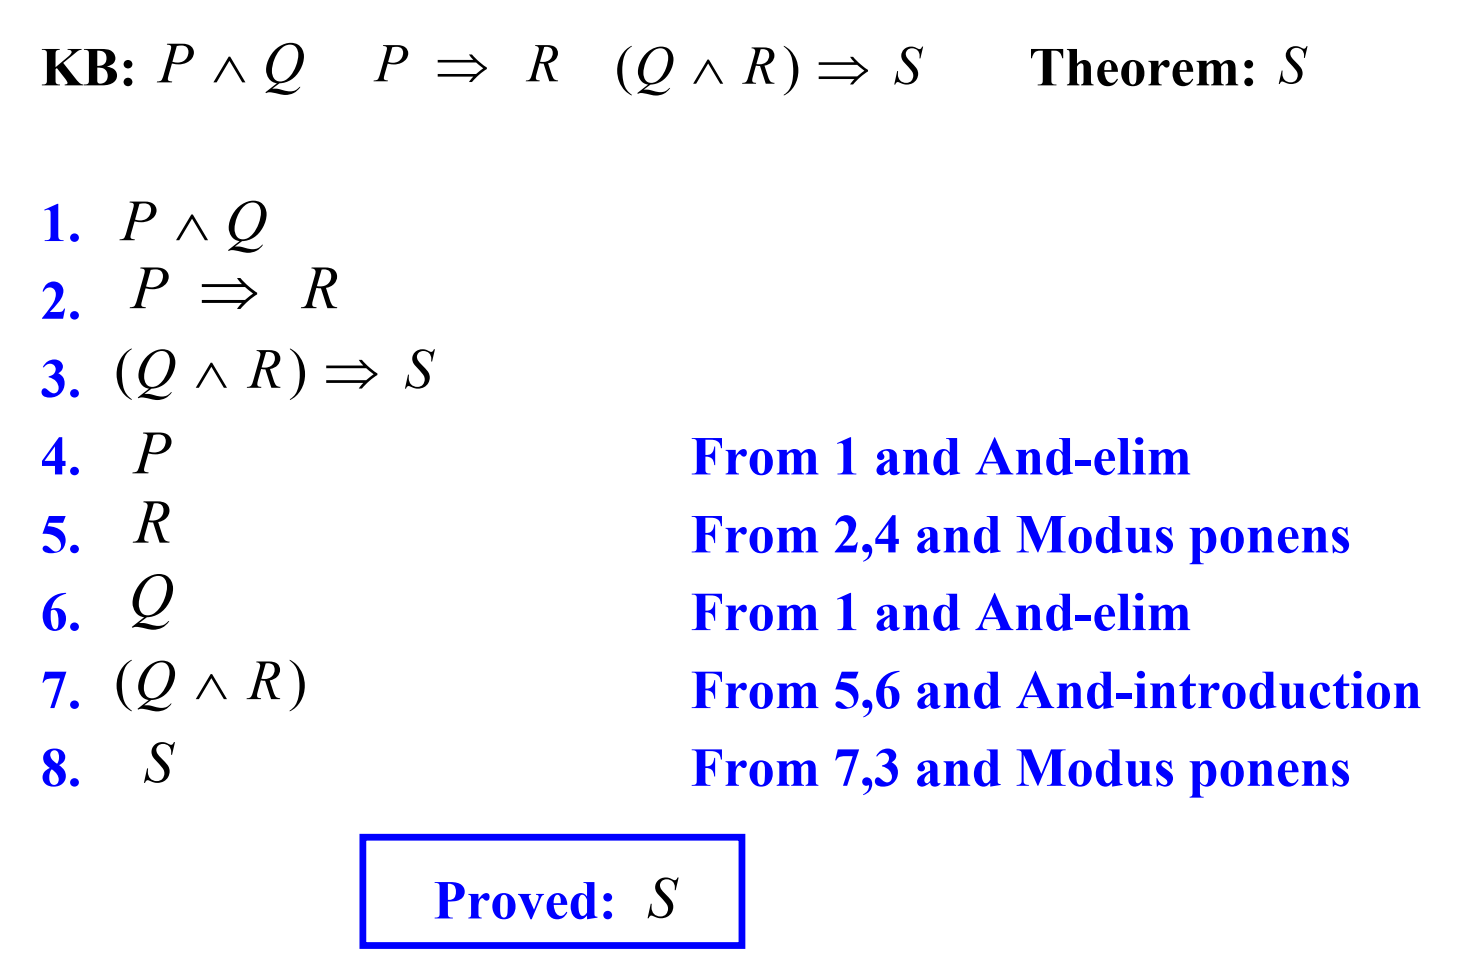
\includegraphics[width=0.4\textwidth]{img/ruleapplication.png}
\end{figure}
This algorithm is sound (inference rules are sound) but it is not complete, unless we define more rules.

There is no way of knowing how many rules do we have to apply or which rule to use at any step.
This can be thought as an instance of a search problem
\subsection{Satisfiability and resolution}
\subsubsection{Validity vs. Satisfiability}
Since we know what we want to prove (i.e we know the Theorem) a clever way would be to find a way to use conclusions in the search for conclusions.

\begin{tcolorbox}[colback=red!5!white,colframe=red!75!black,title=\textbf{Validity Definition}, label=def:validity]
    \label{def:val}
    A formula is valid if it is true in \textbf{all} possible models.
    \begin{equation*}
        \text{For any sentences } \alpha \text{ and } \beta, \alpha \models \beta \text{ if and only if the sentence }\alpha\implies\beta \text{ is valid}
    \end{equation*}
\end{tcolorbox}
\begin{tcolorbox}[label=def:sat,colback=red!5!white,colframe=red!75!black,title=\textbf{Satisfiability Definition}]
    \label{def:sat}
    A formula is satisfiable if it is true in \textbf{at least one} model.
    \begin{itemize}
        \item If f is valid, than the negation of f is unsatisfiable
        \item If f is satisfiable, then the negation of f is invalid
    \end{itemize}
    \begin{equation*}
        \alpha \models \beta \text{ if and only if the sentence }\alpha\land\lnot\beta \text{ is unsatisfiable} \quad \text{\textbf{(Absurdum reduction)}}
    \end{equation*}
    Proving a thesis is equivalent to proving the absurdum of its negation.
\end{tcolorbox}
From Definition of Validity and Satisfiability we can reformulate entailment:
\begin{equation*}
    \alpha\models\beta\;\leftrightarrow\;\alpha\implies\beta\;=\;\lnot\alpha\lor\beta\rightarrow negation \rightarrow \lnot(\lnot\alpha\lor\beta)\rightarrow \alpha\lor\lnot\beta
\end{equation*}
Now we have converted the problem of entailment into proving that a formula is UNSAT.

\subsubsection{Resolution}
Resolution assumes that knowledge base and thesis are expressed in Conjunctive
Normal Form (CNF).
\begin{itemize}
    \item \textbf{Normal form} corresponds to clauses (disjunctions and negations only).
    \item \textbf{CNF} corresponds to conjunction of clauses
\end{itemize}

Resolution Rule: $\inferrule{\{p, q\} \\\\ \{\lnot p,r\}}{\{q, r\}}$

The planning problem can be reformulated as:
\begin{enumerate}
    \item Is the planning problem satisfiable (i.e., is there any feasible sequence of actions)?
    \item Given initial conditions, goal and action rules, what is the next possible action sequence?
\end{enumerate}

Propositional Logic is not enougth:
\begin{itemize}
    \item we also need predicates (functions), not only atoms or variables. To solve this issue we need to intruduce \textbf{First Order Logic (FOL)}
    \item We need to introduce time (one action per time step, or possibly temporal conditions on actions). To solve that we need to introduce \textbf{(Linear) Temporal Logic (LTL)}
\end{itemize}

\subsection{Inference in FOL}
\begin{figure}[H]
    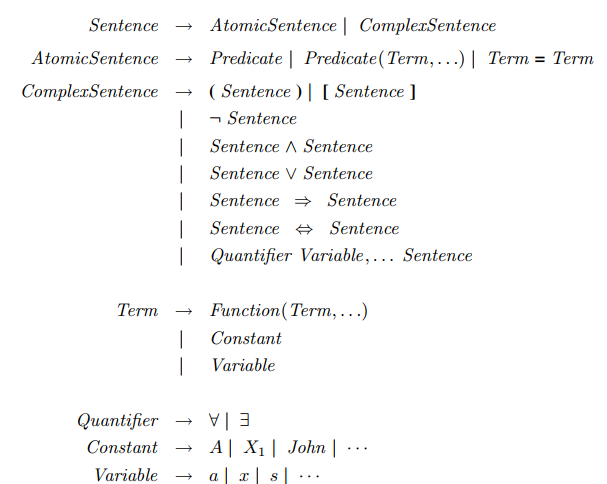
\includegraphics[width=0.5\textwidth]{img/FOL.png}
    \centering
\end{figure}

\textbf{Ground term}: a term which does not contain variables
\begin{itemize}
    \item move(A, B) NOT GROUND $\rightarrow$ no value to vars
    \item move(room1, room2) GROUND $\rightarrow$ value to vars
\end{itemize}

\textbf{Substitution}: replacing a term with another (typically, a variable with a constant)

$\inferrule{\forall v\;\alpha}{Subst(\{v/g\}, \alpha)}\quad \inferrule{\exists v\;\alpha}{Subst(\{v/k\}, \alpha)}$

g = all possible constants (ground terms) for v\\
k = skolem constant\\

For example from the sentence $\exists x Crown(x)\land OnHead(x, Jhon)$ we can infer the sentence:
$Crown(C_1)\land OnHead(C_1, Jhon)$

\subsection{LTL}
\begin{equation*}
    \varphi \coloneqq T \;|\; p \;|\; \lnot\varphi \;|\; \varphi_1 \land \varphi_2 \;|\; \varphi_1 U \varphi_2 \;|\; X\varphi
\end{equation*}
Where $U$ is the Until symbol\\
Where $X$ is the Next symbol\\

\subsection{Logic for explainable agency}
\begin{itemize}
    \item Propositional logic gives the basic syntax and semantics for representing the planning problem
    \item FOL adds hierarchical structure (classes and instances) of real world
    \item LTL adds temporal structure
\end{itemize}
For our purpose this is enougth but if we have more complex problems we may need other stuff:
\begin{itemize}
    \item Stochastic planning domain
    \begin{itemize}
        \item Problabilistic logic
        \item Markov logic networks
    \end{itemize}
    \item The addition of all this stuff might be an issue for complexity
    \begin{itemize}
        \item Decidability:\\
        From PSPACE to EXPSPACE-complete with time\\
        Potentially undecidable with stochasticity
        \item Synthesis is 2EXPTIME-complete with LTL over finite traces
    \end{itemize}
\end{itemize}